%Pakete;
%A4, Report, 12pt
\documentclass[ngerman,a4paper,12pt]{scrreprt}
\usepackage[a4paper, right=20mm, left=20mm,top=30mm, bottom=30mm, marginparsep=5mm, marginparwidth=5mm, headheight=7mm, headsep=15mm,footskip=15mm]{geometry}

%Papierausrichtungen
\usepackage{pdflscape}
\usepackage{lscape}

%Deutsche Umlaute, Schriftart, Deutsche Bezeichnungen
\usepackage[utf8]{inputenc}
\usepackage[T1]{fontenc}
\usepackage[ngerman]{babel}

%quellcode
\usepackage{listings}

%tabellen
\usepackage{tabularx}

%listen und aufzählungen
\usepackage{paralist}

%farben
\usepackage[svgnames,table,hyperref]{xcolor}

%symbole
\usepackage{latexsym,textcomp}
\usepackage{amssymb}

%font
\usepackage{helvet}
\renewcommand{\familydefault}{\sfdefault}

%Abkürzungsverzeichnisse
\usepackage[printonlyused]{acronym}

%Bilder
\usepackage{graphicx} %Bilder
\usepackage{float}	  %"Floating" Objects, Bilder, Tabellen...
\usepackage[space]{grffile} %Leerzechen Problem bei includegraphics
\usepackage{wallpaper} %Seitenhintergrund setzen
\usepackage{transparent} %Transparenz

%for
\usepackage{forloop}
\usepackage{ifthen}

%Dokumenteigenschaften
\title{Summary InfSi1}
\author{Tobias Blaser}
\providecommand{\versionnumber}{1.3}
\date{\today{}, Uster}


%Kopf- /Fusszeile
\usepackage{fancyhdr}
\usepackage{lastpage}

\pagestyle{fancy}
	\fancyhf{} %alle Kopf- und Fußzeilenfelder bereinigen
	\renewcommand{\headrulewidth}{0pt} %obere Trennlinie
	\fancyfoot[L]{\jobname} %Fusszeile links
	\fancyfoot[C]{Seite \thepage/\pageref{LastPage}} %Fusszeile mitte
	\fancyfoot[R]{\today{}} %Fusszeile rechts
	\renewcommand{\footrulewidth}{0.4pt} %untere Trennlinie

%Kopf-/ Fusszeile auf chapter page
\fancypagestyle{plain} {
	\fancyhf{} %alle Kopf- und Fußzeilenfelder bereinigen
	\renewcommand{\headrulewidth}{0pt} %obere Trennlinie
	\fancyfoot[L]{\jobname} %Fusszeile links
	\fancyfoot[C]{Seite \thepage/\pageref{LastPage}} %Fusszeile mitte
	\fancyfoot[R]{\today{}} %Fusszeile rechts
	\renewcommand{\footrulewidth}{0.4pt} %untere Trennlinie
}

\usepackage{changepage}

\newcommand{\important}[1]{
	 \fcolorbox{black}{black}{ %
		\parbox{17cm}{%
			\vspace{0.1cm}
			\hspace{0.1cm}
   			\transparent{1.0}
			\color{white}
			\fontsize{12}{14} \selectfont #1
			\vspace{0.1cm}
   		}
    }
}

\newcommand{\expl}[2]{
	 \fcolorbox{gray}{gray}{ %
		\parbox{17cm}{%
			\vspace{0.1cm}
			\hspace{0.1cm}
   			\transparent{1.0}
			\color{white}
			\fontsize{12}{14} \selectfont #1: #2
			\vspace{0.1cm}
   		}
    }
}

\newcommand{\definition}[2]{
	 \fcolorbox{teal}{teal}{ %
		\parbox{17cm}{%
			\vspace{0.1cm}
			\hspace{0.1cm}
   			\transparent{1.0}
			\color{white}
			\fontsize{12}{14}	
				\selectfont 
			Definition: \\ 
			#1: #2
			\vspace{0.1cm}
   		}
    }
}

%links, verlinktes Inhaltsverzeichnis, PDF Inhaltsverzeichnis
\usepackage[bookmarks=true,
bookmarksopen=true,
bookmarksnumbered=true,
breaklinks=true,
colorlinks=true,
linkcolor=black,
anchorcolor=black,
citecolor=black,
filecolor=black,
menucolor=black,
pagecolor=black,
urlcolor=black
]{hyperref} % Paket muss unbedingt als letzes eingebunden werden!

\usepackage{graphicx}
\begin{document}

% Inhaltsverzeichnis
\tableofcontents
\clearpage

\chapter{W2}

\chapter{W4 (Ch2.2) - Systemprogrammierung}
\definition{Systemprogrammierung}{betriebssystemnahe Programmierung}
\definition{Systemdienstaufruf (System service call)}{Aufrufen einer C-Funktion des Systems}
\begin{figure}[htp]
	\centering
	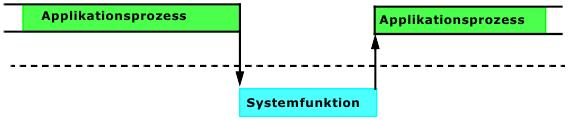
\includegraphics[scale=1.00]{img/w4.1.jpg}
	\caption{}
	\label{}
\end{figure}
\definition{Systemprogrammierschnittstelle}{API des Betriebssystems, eine Sammlung von C-Funktionen}
Oftmals Betrachtung des Betriebsystems als Black Box. 


Systemprogrammierung:
\begin{itemize}
	\item  Nutzung der API des Betriebssystems in Applikationsprogrammen
 	\item Arbeiten mit Beschreibungen von Systemfunktionen (bei der Applikationsentwicklung)
	\item Verwendung einer Programmbibliothek von Systemfunktionen Beispiel: kernel32.dll $\rightarrow$	 Enthält allg. Windows Systemfunktionen
\end{itemize}

\section{Antwortzeit}
\begin{enumerate}
	\item Aufruf einer Systemfunktion: dauert us
	\item Aufruf einer Systemfunktion, die z.B. Hardware anspricht: dauert us bis ms bis ewig
	\item Aufruf einer Systemfunktion die z.B einen Webdienst nutzt: dauert us bis ms bi ewig
\end{enumerate}
Problem: ewiges dauern wird oft in Applikationen vergessen $\rightarrow$ Applikation wartet und reagiert nicht (hängt)

\section{Dienstanforderung und Erbringung}
\begin{figure}[htp]
	\centering
	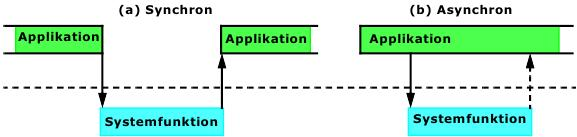
\includegraphics[scale=1.00]{img/w4.2.jpg}
	\caption{}
	\label{}
\end{figure}
\begin{description}
	\item[Synchrone Diensterbringung]
Aufrufer wird für die Dauer der Servicezeit blockiert (d.h. schlafen gelegt)
	\item[Asynchrone Diensterbringung]
Aufrufer kann weiterarbeiten; muss Resultat aber explizit abfragen
\end{description}

\subsection{Zeitüberwachung}
\begin{itemize}
	\item Immer sinnvoll, wenn Servicezeit unbekannt.
	\item Verantwortlich ist der Applikationsentwickler (Zeitüberwachung muss in der Regel explizit programmiert werden).
\end{itemize}

\subsubsection{Programmierung der Zeitüberwachung}
\begin{itemize}
	\item Einfach, falls Systemfunktionen einen Timeout-Parameter unterstützen
	\item Ansonsten nur mit Hilfe zusätzlicher Dienste (systemabhängig)
\end{itemize}

\section{Systemprogrammierschnittstelle}
\subsection{Dienstparameter}
Zusätzliche Informationen die der Dienstanforderung mitgegeben werden und vom Dienst abhängig sind.

\subsubsection{Austausch grosser Datenmengen}
Wichtigster Dienstparameter: Datenort (Spezifizikation des Datenblocks / Puffers $\rightarrow$ Zeiger auf den Anfang) \\
\expl{Plattformunabhängige Grössenangabe}{10*sizeof(int)}
\begin{figure}[htp]
\centering
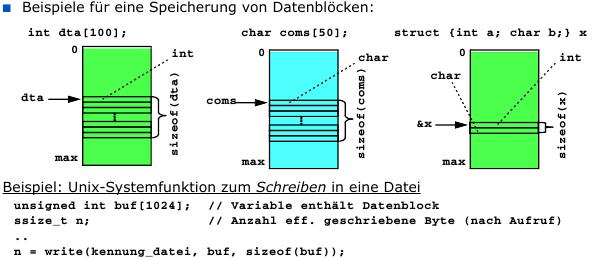
\includegraphics[scale=1.00]{img/w4.3.jpg}
\caption{}
\label{}
\end{figure}
buf darf erst verändert werden, wenn der write-vorgang abgeschlossen ist. \\
Rückgabewert: gibt geschriebene Bytes an.

\subsubsection{Definition von Attributmengen}
\definition{Attribut}{Eigenschaft eines Objektes}
$\rightarrow$ Zusammenfassung mehrere Parameter in einem

Optionen setzen: mit Bitpositionen:
\begin{figure}[htp]
\centering
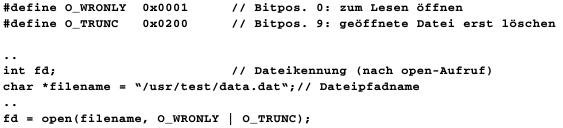
\includegraphics[scale=1.00]{img/w4.4.jpg}
\caption{}
\label{}
\end{figure}

\subsubsection{Strukturierte Dienstparameter}
\begin{itemize}
	\item Zusammenfassen von Dienstparametern mit Struct
	\item Übergeben des Stucts dem Systemlimit als Parameter
\end{itemize}

\section{Systemdatentypen}
\begin{itemize}
	\item  Elementar: int, char, float, double, void, usw.
	\item Abgeleitet: enum, struct, union, Vektor (array), Zeiger (pointer), usw.
\end{itemize}

\subsection{Prinzip der opaken Datentypen}
\begin{itemize}
	\item Interne Struktur soll unsichtbar bleiben (= nicht transparent)
	%\item Tragen eigene Namen, die von den Standarddatentypen abweichen (z.B. pid_t)
	\item Zur Deklaration von Variablen als Behälter (container) von unbekannten Daten
\end{itemize}

\section{Rückgabe der Resultate von Systemfunktionen}
\begin{itemize}
	\item  Rückgabe als Funktionsresultat
	\item Rückgabe über eine oder mehrere vordeklarierte Variablen
	\item Kombination der zwei Möglichkeiten
\end{itemize}

\expl{Rückgabewert C}{struct erlaubt, Array nicht!}

\section{Fehlerbehandlung bei Systemfunktionen}
\begin{itemize}
	\item Systemfunktionen melden mehr oder weniger detailliert Fehler (Ausführung ok oder fehlerhaft, z.T. zusätzlich mit Fehlercode)
	\item Reaktionsmöglichkeiten auf Fehler
		\begin{itemize}
			\item  Ignorieren
			\item Fehlermeldung an Benutzer und Programmabbruch
			\item Fehlermeldung an Benutzer und Wiederholung (Neuversuch)
			\item Fehlermeldung an Benutzer und Frage, wie weiterfahren?
			\item Evtl. Fehlerprotokollierung (für Entwickler)
			\item Evtl. Sicherung von Temporärdaten (für Benutzer)
		\end{itemize}
\end{itemize}



\end{document}
